\capitulo{4}{Técnicas y herramientas}

En esta sección se pretende introducir al lector en algunas de las técnicas y herramientas relevantes en el desarrollo del proyecto.

\section{Técnicas}

Se presentan a continuación algunas de las técnicas más influyentes en materias relacionadas con este trabajo de investigación:

\subsection{CRISP-DM}
Una metodología común, no propietaria y abierta de desarrollo para proyectos de ML es CRISP-DM (Cross-Industry Standard Process for Data Mining). Nacida del trabajo conjunto de un grupo de empresas, consta de un proceso iterativo y adaptable.

Sin pretender desarrollar exhaustivamente la misma, se muestra a continuación un resumen de sus 6 principales fases~\cite{apuntesSisint}.

\begin{enumerate}
	\item \textbf{Compresión del negocio:} el objetivo de esta fase es entender los requerimientos del proyecto observados bajo un prisma empresarial y aplicar dicho conocimiento a la definición del problema de minería de datos.
	
	\item \textbf{Compresión de los datos:} consiste en recopilar y explorar los datos con el objetivo de conocerlos. También se pretende identificar problemas de calidad y posibles subconjuntos de datos con especial interés para ser analizados.
	
	\item \textbf{Preparación de los datos:} se busca procesar el conjunto de datos seleccionado con el fin de ser utilizable en algoritmos de ML. Por lo tanto, se incluyen todas las tareas de adecuación de los datos al problema de aprendizaje que se consideren necesarios.
	
	\item \textbf{Modelado:} en esta fase se pretende aplicar las técnicas de ML seleccionadas a las vistas obtenidas anteriormente, y se evalúa utilizando técnicas específicas de aprendizaje. 
	
	\item \textbf{Evaluación:} a diferencia de la fase anterior, se busca evaluar el modelo desde el punto de vista del objetivo del negocio. Es decir, determinar si responde ante los objetivos empresariales planteados con anterioridad.
	
	\item \textbf{Despliegue y explotación:} en la última fase, se integran los modelos en los procesos de la organización y se aprovecha el conocimiento generado.
\end{enumerate}

Es relevante destacar la naturaleza cíclica y no rígida de la metodología, permitiendo que algunas fases alimenten sus predecesoras o que incluso algunos proyectos motiven el lanzamiento de otros.

\subsection{DevOps y CI/CD}

CI/CD (\textit{continuous integration and continuous delivery}) se refiere al conjunto de prácticas de desarrollo que permite la entrega rápida y fiable de código gracias a la automatización de procesos~\cite{cdciUnity}, mientras que DevOps es la cultura que engloba estas prácticas buscando lograr un desarrollo de \textit{software} más eficaz. El ciclo de vida se muestra en la imagen~\ref{img:4_cicd}.

\begin{figure}[h]
	\caption[Técnicas: Ciclo de vida del CI/CD]{Representación del ciclo de vida del CI/CD. Extraída de: \url{https://es.parasoft.com/blog/implementing-qa-in-a-ci-cd-pipeline/}}
	\centering
	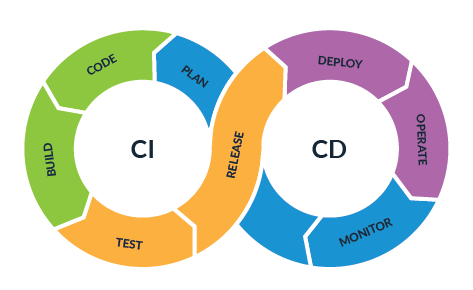
\includegraphics[scale=0.6]{../img/memoria/4_cicd.png}
	\label{img:4_cicd}
\end{figure}


CI (integración continua) es la práctica que permite integrar repetidas veces en pequeños segmentos temporales cambios en un repositorio de código. En este proyecto, para garantizar que los nuevos cambios introducidos en el repositorio son seguros y el \textit{merge} de las nuevas ramas no va a perjudicar versiones anteriores de código, se han automatizado distintos procesos (ejecución automática de \textit{test}, análisis de código, escáneres de filtraciones de credenciales, etc.) utilizando las herramientas descritas en la sección~\ref{sec:herramientas_control_calidad}. Por otro lado, la entrega continua automatiza el despliegue de código a los usuarios finales, liberando a los equipos de operaciones de procesos manuales~\cite{cdciRedHat}. 

DevOps, sin embargo, abarca más. Esta cultura busca cubrir el ciclo completo del desarrollo de \textit{software}, desde la estructura del equipo hasta el control de versiones, y se sirve de las prácticas de CI/CD para lograr este fin.

\subsection{Gitflow}

Gitflow es un modelo alternativo de creación de ramas. Se caracteriza por contar con ramas de función y ramas principales, siendo recomendable aplicarlo en proyectos que trabajen con CD/CI~\cite{gitFlow}. En concreto, han sido utilizadas ramas principales y de desarrollo, fusionando el resultado de ésta última al final de cada \textit{sprint}. Debido a que en el equipo trabaja un único desarrollador, se ha desestimado crear una rama por \textit{feature} lanzada. Para garantizar que los \textit{merge} a la rama principal son seguros, se ha automatizado el uso de las herramientas desarrolladas en la sección~\ref{sec:herramientas_control_calidad}, generando \textit{builds} cada vez que se integra una rama nueva.

\subsection{Scrum}

Scrum es una metodología ágil basada en cuatro valores~\cite{scrumMaster2022}. Sintetizando sus principios, se puede deducir que se pretende valorar a los individuos por encima de las herramientas, el software apropiado a la documentación exhaustiva, la colaboración con el cliente y la habilidad de dar respuesta al cambio ante imprevistos.

Se describe en profundidad este método y cómo se ha desarrollado el trabajo siguiendo sus principios en los anexos.

\subsection{\textit{Web Scraping}}

Web scraping es una técnica de extracción de datos que consiste en automatizar el proceso de recolección de información de sitios \textit{web}~\cite{webScraping}.

En este trabajo ha sido empleado para extraer la información necesaria para generar vectores de características (consultar~\ref{sec:vectores_caracteristicas_phishing}) para cada una de las URL en el \textit{dataset} (consultar~\ref{ss:extracción-dataset-phishing}). Para ello, se ha utilizado la librería Requests de Python, realizando peticiones HTTP a los enlaces y obteniendo el código HTML de la página en respuesta para ser analizado automáticamente.

\section{Herramientas}

Se muestra a continuación algunas de las herramientas más relevantes en el desarrollo del proyecto.

\subsection{Librerías}

Principalmente de Python, se destacan las siguientes utilidades:

\begin{itemize}
	\item \textbf{Scikit-Learn}: una de las librerías referentes en el ámbito de \textit{machine learning} y Python. Además de utilizar la vertiente relacionada con aprendizaje automático, también se aprovecharon otras ramas del módulo como la de extracción de características de texto (TF-IDF)~\cite{sslearnRepo}. Debido a que proporciona una interfaz estándar para los clasificadores base de muchos algoritmos, posee muy buena documentación y es compatible con otras librerías, ha sido muy utilizada.
	
	\item \textbf{sslearn}: librería desarrollada por José Luis Garrido-Labrador dedicada al aprendizaje semisupervisado en Python. Utilizada para realizar comparaciones con algunos de los algoritmos implementados~\cite{sslearnRepo}.
	
	\item \textbf{LAMDA}: \textit{toolkit} escrito en Python con algunas implementaciones de los algoritmos más relevantes de aprendizaje semisupervisado~\cite{lamdasslRepo}. Nuevamente, ha sido utilizada como referente a la hora de realizar comparaciones contra las implementaciones propias~\cite{lamdasslPaper}.
	
	\item \textbf{Beautiful soup}: biblioteca de Python utilizada para extraer datos de ficheros \texttt{HTML} obtenidos mediante la realización de \textit{web scraping} a la hora de sintetizar vectores de características para la detección de \textit{phishing}. Se ha recurrido a ella, principalmente, cuando la obtención de ciertos campos en las etiquetas puede ser vulnerada mediante el uso de expresiones regulares corrientes~\cite{bs4Docs}.
	
	\item \textbf{TLD}: librería de Python utilizada para extraer dominios de alto nivel (TLDs) de los enlaces facilitados~\cite{tldLibreria}. Para evitar dependencias de biblitecas externas, en un primer momento se consideró trabajar con una lista del \textit{top} dominios más comunes (extraída de~\cite{tldLista}). Sin embargo, se descartó la idea debido a que no existe una forma intrínseca de saber qué cadenas son TLD y cuales son subdominios. Por ejemplo, \texttt{zap.co.it} es un subdominio ya que existe el TLD \texttt{co.it}. Sin embargo, en un país que no venda dominios de la forma \texttt{co.<<pais>>} sería un TLD~\cite{tldNogenerico}.
	
	\item \textbf{NLTK}: \textit{toolkit} de Python utilizado para trabajar con lenguaje natural. Su principal utilidad ha sido procesar palabras como \textit{tokens} para poder facilitar la implementación de algoritmos más complejos como TD-IDF o para analizar y procesar texto~\cite{nltk}.
	
	\item \textbf{Otros}: otras de las dependencias (estándar) del proyecto se enumeran a continuación.
		\begin{itemize}
			\item \textbf{Requests}: permite realizar peticiones a distintas URLs, además de especificar parámetros relevantes en las mismas (como \textit{headers}, \textit{cookies}, \textit{proxies} o \textit{timeouts}).
			\item \textbf{urllib}: procesa URLs y las divide en campos.
			\item \textbf{re}: utilizada para aplicar expresiones regulares en Python.
			\item \textbf{Numpy, Pandas, Matplotlib}: utilizadas para tratar vectores, operaciones en \textit{arrays}, \textit{dataframes} y representar resultados.
		\end{itemize}	
\end{itemize}



\subsection{Extensiones y portales}

Principalmente utilizados para control de versiones, realización de \textit{test} y seguimiento de la metodología Scrum, se encuentran:

\begin{itemize}
	\item \textbf{ZenHub}: extensión dedicada a la gestión de proyectos \textit{software} que se integra directamente con Github. Permite visualizar proyectos, \textit{sprints}, gráficos propios de Scrum y crear tableros. Debido a que el equipo de desarrollo cuenta con un único integrante, se considera la alternativa óptima (por ejemplo, a Jira) por su sencillez~\cite{zenhubHome}.
	
	\item \textbf{Selenium IDE}: herramienta de automatización que permite grabar, editar y depurar pruebas, además de exportarlas a algunos de los lenguajes de programación más comunes. En concreto, se ha utilizado la extensión para navegadores Selenium IDE, que consiste en un entorno de pruebas \textit{software} para \textit{webs} que permite grabar y reproducir \textit{test} paso a paso sin necesidad de programar~\cite{seleniumIDE}.
	
	\item \textbf{GitHub}: portal que permite alojar distintos repositorios en la nube~\cite{githubHome}. Ha sido escogido por ser una de las plataformas más populares, además de por permitir la interacción entre distintos usuarios. La gestión del \textit{backlog} del producto ha sido simulada mediante la creación de \textit{issues}.
	
	\item \textbf{Pandoc}: conversor de documentos de código abierto~\cite{pandoc} utilizado para convertir \LaTeX{} en HTML y facilitar la escritura de la \textit{wiki} del repositorio\footnote{Disponible en \url{https://github.com/phf1001/semisupervised-learning-in-cibersecurity/wiki}}.
\end{itemize}

\subsection{Programas}

En versión de escritorio, únicamente ha sido necesario recurrir a:

\begin{itemize}
	\item \textbf{KEEL}. herramienta desarrollada en Java por distintas universidades españolas y financiada por el Ministerio de Educación y Ciencia~\cite{keelRepo}. Proporciona implementaciones de \textit{machine learning}, y ha sido utilizada para probar aquellos algoritmos no disponibles en las librerías de Python mencionadas anteriormente.
	\item \textbf{\TeX{}Studio}
	Editor de \LaTeX{} utilizado.
	\item \textbf{Git BASH}
	Emulador de BASH para Microsoft Windows que proporciona una terminal de línea de comandos de Git.
	\item \textbf{Notion}: organizador de tareas multiplataforma utilizado para tomar notas, planificar temporalmente el trabajo y contabilizar el número de horas dedicadas al proyecto~\cite{notion}.
\end{itemize}


\subsection{Entorno de programación}

Relativo a la creación de un entorno que pueda ser reproducible, se facilita la siguiente información:

\begin{itemize}
	\item \textbf{Python}: lenguaje de programación interpretado de propósito general. Ha sido escogido para realizar este proyecto debido a la gran cantidad de paquetes dedicados a la ciencia de datos que posee~\cite{python}.
	\item \textbf{Visual Studio Code}: editor y depurador de código empleado junto a algunas de sus principales extensiones.
	\item \textbf{Entornos virtuales}: un entorno virtual es un directorio que contiene una instalación concreta de Python y los paquetes que se hayan decidido instalar~\cite{venvs}. Como se puede deducir, la correcta utilización de los entornos virtuales conlleva muchas ventajas, como tener varios paquetes sin conflictos entre ellos o evitar corromper la instalación base si se está probando algún elemento nuevo.
	\item \textbf{Conda}: es un sistema de gestión de paquetes y entornos \textit{opensource}. Es especialmente útil a la hora de realizar trabajos de ML ya que posee librerías como SciPy y TensorFlow~\cite{conda}.
\end{itemize}

\subsection{Control de calidad}
\label{sec:herramientas_control_calidad}

Siguiendo los principios de CD/CI, se ha procurado garantizar la calidad del código desarrollado. Para ello se han utilizado diversas herramientas, entre ellas:

\begin{itemize}
	\item \textbf{SonarCloud}: se trata de un servicio de análisis estático de código que notifica diversos parámetros a revisar como \textit{codesmells}, \textit{bugs} o vulnerabilidades. Se ha integrado en el repositorio con la intención de realizar código limpio y aumentar la calidad del proyecto~\cite{sonarCloud}.
	\item \textbf{DeepSource}: se trata de una plataforma que fusiona el análisis estático de código, SAST (\textit{static application security testing}), cobertura de código, entre otros, para mejorar la calidad de los proyectos. Además, posee un \textit{bot} que realiza ciertas correcciones automáticas (por ejemplo, modifica errores de documentación) y facilita \textit{badges}\footnote{Un \textit{badge} o insignia es una imagen que muestra el estado de un flujo de trabajo o un repositorio. Por ejemplo, una insignia para los defectos de código muestra visualmente el número de \textit{code smells} que hay en un determinado proyecto.} para los repositorios~\cite{deepSourceBot}.
	\item \textbf{Travis CI}: se ha utilizado el servicio para la realización automática de \textit{test} cada vez que se actualiza el repositorio. Para ello, se ha configurado una \textit{build} y recreado el entorno del programador. De este modo, antes de realizar un \textit{merge} a la rama principal se puede comprobar rápidamente si las pruebas siguen pasando, lo que mejora la integración y despliegue continuo~\cite{travisCI}.
	\item \textbf{Git Guardian}: herramienta que escanea los repositorios en busca de posibles filtraciones de credenciales, se ha utilizado para garantizar que las contraseñas de acceso a bases de datos y otros secretos permanezcan ocultos. Ha sido incluida, junto con las anteriores, en el flujo de Git~\cite{gitGuardian}.
\end{itemize}

\subsection{Desarrollo \textit{web}, persistencia y despliegue}
\label{sec:despliegue}

\begin{itemize}
	\item \textbf{Flask}: \textit{framework} que permite desarrollar páginas \textit{web} utilizando Python~\cite{flask}. Además, permite la instalación de \textit{plugins} para aumentar su funcionalidad (como, por ejemplo, flask-WTF para gestionar formularios o flask-login para el manejo de sesiones). 
	\item \textbf{Babel}: extensión de Flask utilizada para internacionalizar la aplicación \textit{web} desarrollada~\cite{flaskBabel}. En concreto, la funcionalidad principal utilizada ha sido la traducción mediante archivos \texttt{.pot}, \texttt{.po} y \texttt{.mo}.
	\item \textbf{Jinja2}: motor de plantillas utilizado para generar páginas HTML~\cite{jinja}.
	\item \textbf{Argon Dashboard}: plantilla empleada como base para la \textit{web}\footnote{Disponible en \url{https://github.com/creativetimofficial/argon-dashboard}}.
	\item \textbf{PostgreSQL}: base de datos relacional utilizada debido a su carácter \textit{open source} y disponibilidad multiplataforma.~\cite{postgresql}.
	\item \textbf{SQLAlchemy}: librería utilizada como ORM (\textit{object-relational mapper}). Es decir, permite trabajar con objetos y gestiona su traducción a SQL de forma transparente al programador.~\cite{SQLAlchemy}.
	\item \textbf{Heroku}: solución de plataforma como servicio (PaaS) basada en la nube que gestiona la infraestructura de las aplicaciones desplegadas (en este caso, Krini\footnote{Disponible en \url{https://krini.herokuapp.com/index}})~\cite{heroku}.
	\item \textbf{Gunicorn} servidor web HTTP para aplicaciones Python.~\cite{gunicorn}. Cabe destacar que es fundamental su correcta configuración para evitar errores de concurrencia~\cite{herokuPreload}.
	\item \textbf{Docker}: plataforma de contenedores que simplifica la implementación y gestión de aplicaciones en cualquier entorno.~\cite{docker}.
\end{itemize}

\subsection{\textit{Scripts}} 

En algunos casos no se han encontrado soluciones de terceros y ha sido necesario implementar \textit{scripts} propios. Los mas relevantes se citan a continuación:

\begin{itemize}
	\item \textbf{\textit{Script} para levantar proxies \texttt{SOCKS5}}:
	\label{sec:script_tor}
Durante la extracción de vectores de características, se realizan peticiones a páginas de \textit{phishing}. Para garantizar que estas páginas no puedan rastrear desde donde se ha realizado la petición, se han utilizado \textit{proxies} que implementan el protocolo \texttt{SOCKS5}.

Para ello, se ha implementado en Python un \textit{script} auxiliar que levanta en paralelo tantas instancias de Tor como se soliciten, y mantiene los hilos vivos hasta que se interrumpa la ejecución del \textit{script}.

Por cada instancia de Tor que se quiera levantar, se necesita un fichero \texttt{torrc} en el directorio \texttt{/etc/tor/}~\cite{TorFicherosTor}. Cada una de ellas debe tener, además, su propio puerto de control, su propio puerto \textit{socks} y su directorio de datos. Por ello, se ha creado una clase auxiliar que genera estos ficheros. Para levantar la instancia simplemente ha de ejecutarse el comando \texttt{tor -f /etc/tor/torrc.x} (siendo $x$ el número de la instacia correspondiente), aunque se ha decidido, además, dirigir la salida al fichero \texttt{/dev/null}. Es importante destacar que el puerto de control debe ser el siguiente al puerto \textit{socks}. Teniendo en cuenta que los puertos por defecto de Tor son el 9050 y el 9051, se puede incrementar partiendo de esos números\footnote{Solución basada en la respuesta del usuario <<zkilnbqi>> en Stack Overflow \url{https://stackoverflow.com/questions/14321214/how-to-run-multiple-tor-processes-at-once-with-different-exit-ips}.}. Para comprobar que la instancia levantada funciona correctamente, se hace una petición a \url{http://ipinfo.io/ip} y se comprueba con una expresión regular que la dirección obtenida es la correcta. De este modo, se sabe que el \textit{proxy} HTTP levantado funciona, y se puede utilizar redireccionando las peticiones oportunas a través del \textit{proxy} \texttt{socks5h://127.0.0.1:$y$} (donde $y$ es el puerto \textit{socks} de la instancia correspondiente). Para que pueda ser usado en código, se ha generado un \texttt{JSON} donde se incluyen como diccionarios los \textit{proxies} disponibles, y se utilizan en combinación con la biblioteca Requests.

Debido a que el puerto Tor queda <<a la escucha>> en la máquina local (está esperando que se realice una conexión), no conlleva ningún riesgo. Para cerrar el puerto, es suficiente con parar el proceso que esté ejecutando el \textit{script}. Se puede comprobar ejecutando en una terminal el comando \texttt{sudo lsof -i:$y$} (nuevamente, $y$ es el puerto \textit{socks} levantado). Cuando el \textit{script} esté funcionando, la salida del comando mostrará diversos campos, como el propio comando (Tor), el PID, el nombre (\textit{listen}). Si el \textit{script} se para, el comando no mostrará salida, lo que implica que el puerto no está abierto~\cite{checkOpenTorPorts}.

\item \textbf{\textit{Script} de búsqueda de protocolos y análisis de lenguaje}: utilizado para buscar el protocolo de todas las páginas que forman el \textit{dataset} de URLs legítimas y seleccionar aquellas escritas en inglés y español (consultar sección~\ref{ss:extracción-dataset-phishing}).

\item \textbf{\textit{Scripts} de despliegue en Docker}: facilitados para que los interesados en desplegar la \textit{web} en local puedan hacerlo sin conocimiento de Docker. Disponibles tanto en formato \texttt{.bat} como \texttt{.sh}.

\end{itemize}